\documentclass[12pt,a4paper]{scrartcl}
\usepackage{geometry}
\usepackage{fancyhdr}
\usepackage{url}
\usepackage{csquotes}
\usepackage{graphicx}
\usepackage{amsmath}
\usepackage{amsthm}
\usepackage{amssymb}
\pagestyle{fancy}
\cfoot{\thepage}
\title{Detailed Dissertation Proposal}
\subtitle{Distributed financial data forecaster}
\author{Wang Youan\\{\small Supervised by: YIP Chi Lap}}
\date{\today}
\geometry{left=2cm, right=2cm, top=2cm, bottom=2cm}
\bibliographystyle{ieeetr}
\graphicspath{{images/}}
\begin{document}
	\maketitle
	\section{Introduction}
	This thesis consists of two parts, one is about financial data forecast, the other is about distributed computing.
	\subsection{Financial data forecast}
	Financial data forecast is very important for making business activity planning. The expectation of some financial data such as stock prices will highly affect future price\cite{Mastering_Financial_Calculations} and investors’ behaviors. Besides, recently, algorithmic trading (AT for short) has become more and more important. AT \textquote{is the computerized executions of financial instruments}\cite{kissell2006algorithmic}. Over half of all stocks traded in the US and EU are handled by those systems\cite{nuti2011algorithmic}. And the core of every AT system is financial data forecast, which leads to growing importance of this topic.\\
	There are three types of techniques used in algorithm trading\cite{nuti2011algorithmic},
	\begin{itemize}
		\item \textbf{Fundamental analysis}\cite{lee2006encyclopedia} is a technique that uses underlying factors about given company to determine its stock price. Such aspects may include interest rates, revenue, industry, and etc. The primary notion of fundamental analysis is that the stock price of a certain company will eventually reflect all such factors.
		\item \textbf{Technical analysis}\cite{nuti2011algorithmic} relays on the historical trading price and volume to predict stock price movement. \enquote{Using charts, technical analysts seek to identify price patterns and market trends in financial markets and attempt to exploit those patterns}\cite{murphy1999technical}. In other words, different from fundamental analysis, technicians only concern about the market’s price changes. Technical traders’ mainly tools are various indicators, overlays and charts. Such tools includes MACD (Moving Average Convergence/Divergence Oscillator), RSI (Relative Strength Index), OHLC charts, Fibonacci ratios, etc.  
		\item \textbf{Quantitative analysis}\cite{nuti2011algorithmic} mainly focuses on the stochastic behavior of asset prices. This type of analysis uses more statistical analysis to describe the randomness of a stock price and is used to determine some financial derivative product price such as futures and swaps.
	\end{itemize}
	This dissertation tries to combine technical and fundamental analysis together to predict stock price. I will use some indicators or machine learning algorithms to do the technical part and use Google trend or Yahoo finance to do the financial part. 
	\subsection{Distributed Computing}
	Another important topic is about distributed computing. \enquote{\textit{Distributed system} is a software system in which components located on networked computers communicate and coordinate their actions by passing messages.}\cite{coulouris2012distributed} \textit{Distributed computing} is computing running on a distributed system. Such computing haves below advantages\cite{mahajan2013distributed},
	\begin{itemize}
		\item \textbf{Resource sharing.} A distributed system allows sharing of certain hardware, such as memory, CPU, etc. 
		\item \textbf{Fault Tolerance.} In a distributed system, usually there are certain amount of redundancy. Even if some components errors or failures happened, the system still can function with reduced capacity.
		\item \textbf{Scalability.} Different from monolithic computing, which the limitation of one computer's capacity, distributed computing can be easily upgraded with addition resources.
		\item \textbf{Better price-performance ratio.} With the advance in microprocessors and communication technique, distributed systems have a better price-performance ration than monolithic ones.
	\end{itemize}
	This dissertation uses \textbf{Apache Spark} to implement this forecaster. Spark\cite{karau2015learning} is an open source cluster computing framework. The reason why choosing Spark is that it allows \enquote{programs to load data into a cluster's memory and query it repeatedly}, which makes Spark well-suited to machine learning algorithms
	\section{Objectives}
	One objective of this thesis is to design a stock prices prediction system, whose input is some historical data such as stock prices, trading volume or news related to that company. The finished product will be runs on a distributed system based on Spark. \\
	Another deliverable will be sets of financial data and a method to obtain these data.
	\section{Scope}
	This dissertation will cover the following areas:
	\begin{itemize}
		\item Financial data processing
		\item Market Analysis
		\item Distributed computing
		\item Data Mining
		\item Machine learning
	\end{itemize} 
	\section{Time Schedule}
	This dissertation will be finished within two semesters, i.e., before the end of July. Detailed time schedule can be found in figure~\ref{fig:sche}.
	\begin{figure}[h]
		\centering
		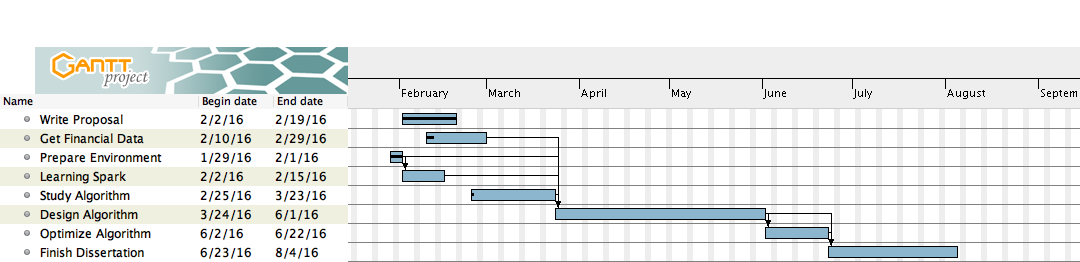
\includegraphics[width=\textwidth]{Schedule.png}
		\caption{Time Schedule}
		\label{fig:sche}
	\end{figure}
	And the detailed estimated number of learning hours for each milestone in the dissertation work is as below,
	\begin{itemize}
		\item Write Proposal: 15hrs
		\item Get Financial Data: 10hrs
		\item Learning Spark: 25hrs
		\item Study Algorithm: 120hrs
		\item Design Algorithm: 160hrs
		\item Optimize Algorithm: 130hrs
		\item Finish Dissertation: 140hrs
	\end{itemize}

	\bibliography{Proposal}
\end{document}